\section{拉普拉斯逆变换}

本节介绍拉普拉斯逆变换。
由于从定义上iLT非常难解,而实际中多数LT的形式是有理式,这里只针对有理式的形式给出留数解。

本节要点:
\begin{itemize}
    \item 了解拉普拉斯逆变换的留数解;
    \item 了解极点类型对逆变换的影响;
    \item 掌握通过极点类型判断逆变换形状。
\end{itemize}

%============================================================
\subsection{有理式、零点和极点}

\begin{definition}
如果信号$x\left( t \right) $的LT可以表达为一个有理式:
\[
X\left( s \right) =\frac{B\left( s \right)}{A\left( s \right)}=\frac{b_ms^m+\cdots +b_1s+b_0}{a_ns^n+\cdots +a_1s+a_0}
\]
\begin{itemize}
    \item $b_i,a_i\in \mathbb{R} $:实系数,且$b_m,a_n\ne 0$;
    \item $m,n\in \mathbb{Z} ^+$:正整数,特别地称{\bf $n$为$X\left( s \right) $的阶数};
    \item $B\left( s \right) ,A\left( s \right) $:{\bf 分子多项式}(numerator polunomial)和{\bf 分母多项式}(denominator polynomial),且它们无公因式。
\end{itemize}
将$A\left( s \right) $化成多项式:
\[
A\left( s \right) =a_n\prod_{i=1}^n{\left( s-p_i \right)}
\]
其中$p_i\in \mathbb{C} $为$A\left( s \right) =0$的根,称为{\bf $A\left( s \right) $的零点}。
如果某一个零点是复数,则其共轭复数也是零点,也即复数零点成共轭对出现。
相应的LT可写为:
\[
X\left( s \right) =\frac{B\left( s \right)}{a_n\prod_{i=1}^n{\left( s-p_i \right)}}
\]
此时,$p_i$也称为{\bf $X\left( s \right) $的极点}。
$A\left( s \right) =0$也可称为{\bf 系统的特征方程},$p_i$也称{\bf 系统的特征根}。
\end{definition}

$p_i$对于$A\left( s \right) $称为零点,对于$X\left( s \right) $称为极点,对于系统称为特征根。
所有项中,我们最关心$p_i$,它决定了系统的稳定性。

%============================================================
\subsection{Python应用——numpy.roots函数}

Numpy中的roots函数求解多项式的根。
\begin{figure}[ht]
\centering
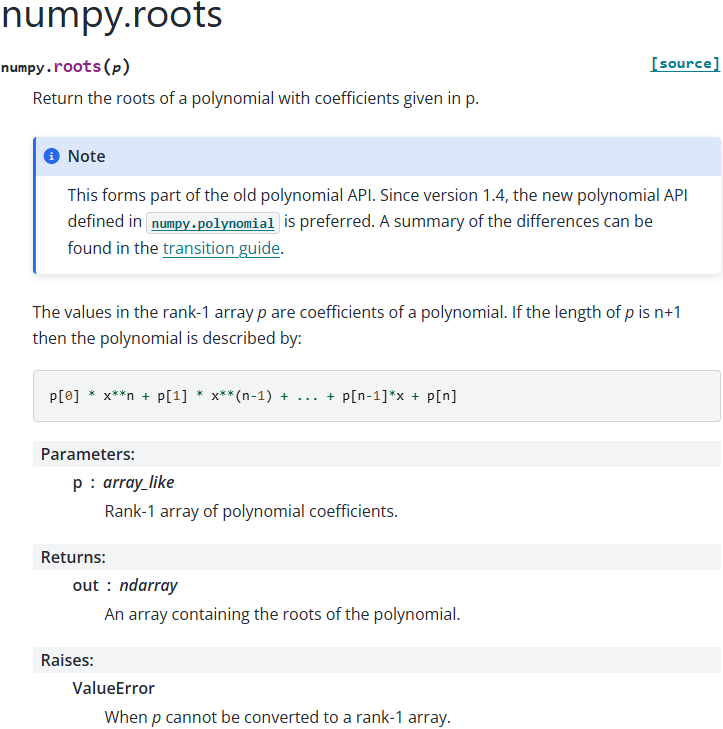
\includegraphics[width=10cm]{7.2.2-1.png}
\end{figure}

~

\begin{example}
如有多项式$A\left( s \right) =s^3+4s^2+6s+4$,求根。
\end{example}

\begin{python}
>>> import numpy as np
>>> p = np.roots([1, 4, 6, 4])
>>> p
array([-2.+0.j, -1.+1.j, -1.-1.j])
\end{python}

%============================================================
\subsection{iLT的留数解——单极点}

设LT变换:
\[
X\left( s \right) =\frac{B\left( s \right)}{A\left( s \right)} \qquad m<n
\]
若有{\bf 单极点}(distinct pole,即$p_i\ne p_j$),用留数方法求解拉普拉斯逆变换,步骤如下:
\begin{enumerate}
    \item 首先求得极点$p_i$的值,于是LT可化为极点的和式:
    \[
    X\left( s \right) =\sum_{i=1}^n{\frac{c_i}{s-p_i}}=\frac{c_1}{s-p_1}+\frac{c_2}{s-p_2}+\cdots +\frac{c_n}{s-p_n}
    \]
    \item 求得留数$c_i$:
    \[
    c_i=\left. \left[ \left( s-p_i \right) X\left( s \right) \right] \right|_{s=p_i}
    \]
    \item 由于LT的线性性,可得逆变换:
    \[
    x\left( t \right) =\sum_{i=1}^n{c_ie^{p_it}}=c_1e^{p_1t}+c_2e^{p_2t}+\cdots +c_ne^{p_nt} \qquad t\geqslant 0
    \]
\end{enumerate}
注意:
\begin{itemize}
    \item 如果单极点是实数,则留数也是实数,iLT结果的对应项是$ce^{p_it}$,表示时域呈指数发散或收敛;
    \item 如果单极点有复数,则必以共轭对$p_i,\bar{p}_i=\sigma \pm i\omega $的形式出现,对应留数也有共轭对$c_i,\bar{c}_i$,此时,时域中的共轭对必能合并为实数项$c_ie^{p_it}+\bar{c}_ie^{\bar{p}_it}=2\left| c_i \right|e^{\sigma t}\cos \left( \omega t+\angle c_i \right) $,表示以指数包络振荡;
    \item 如果单极点是纯虚数$\sigma =0$,也是共轭对$p_i,\bar{p}_i=\pm i\omega $,iLT结果项为$2\left| c_i \right|\cos \left( \omega t+\angle c_i \right) $,表示时域稳定震荡。
\end{itemize}

\begin{tcolorbox}
可结合微积分中的二阶微分方程理解iLT的收敛项和振荡项。
\end{tcolorbox}

%============================================================
\subsection{iLT的留数解——重复极点}

若拉普拉斯变换如下:
\[
X\left( s \right) =\frac{c_1}{s-p_1}+\frac{c_2}{\left( s-p_1 \right) ^2}+\frac{c_3}{\left( s-p_1 \right) ^3}+\cdots +\frac{c_r}{\left( s-p_1 \right) ^r}+\cdots
\]
极点$p_1$有$r$次重复,相应的留数:
\[
c_i=\frac{1}{\left( r-i \right) !}\cdot \left. \left[ \frac{d^{r-i}}{ds^{r-i}}\left[ \left( s-p_1 \right) ^rX\left( s \right) \right] \right] \right|_{s=p_1} \qquad i=1,2,\cdots ,r
\]
即:
\begin{align*}
&c_1=\frac{1}{\left( r-1 \right) !}\cdot \left. \left[ \frac{d^{r-1}}{ds^{r-1}}\left[ \left( s-p_1 \right) ^rX\left( s \right) \right] \right] \right|_{s=p_1} \\
&c_2=\frac{1}{\left( r-2 \right) !}\cdot \left. \left[ \frac{d^{r-2}}{ds^{r-2}}\left[ \left( s-p_1 \right) ^rX\left( s \right) \right] \right] \right|_{s=p_1} \\
&\vdots \\
&c_{r-2}=\frac{1}{2!}\cdot \left. \left[ \frac{d^2}{ds^2}\left[ \left( s-p_1 \right) ^rX\left( s \right) \right] \right] \right|_{s=p_1} \\
&c_{r-1}=\left. \left[ \frac{d}{ds}\left[ \left( s-p_1 \right) ^rX\left( s \right) \right] \right] \right|_{s=p_1} \\
&c_r=\left. \left[ \left( s-p_1 \right) ^rX\left( s \right) \right] \right|_{s=p_1}
\end{align*}
再根据LT性质$\frac{t^{n-1}}{\left( n-1 \right) !}e^{-at}\leftrightarrow \frac{1}{\left( s+a \right) ^n}$即可得到iLT的对应项。
这种情况下,信号会包含$t$的次方的多项式。

%============================================================
\subsection{iLT的留数解——总结}

极点类型及数量决定了时域的形状(收敛、发散、振荡),分子多项式$B\left( s \right) $不影响的形状,只影响留数$c_i$的值。
\begin{table}[h]
\centering
% \caption{表头}
\begin{tabular}{ccc}
    \toprule
    极点类型 & 时域包含项 & 物理意义\\
    \midrule
    实数单极点 & $ce^{pt}$ & 增益项\\
    复数单极点 & $2\left| c \right|e^{\sigma t}\cos \left( \omega t+\angle c \right) $ & 振荡项\\
    重复点 & $c_1e^{pt}+c_2te^{pt}+c_3t^2e^{pt}+\cdots $ & \\
    \bottomrule
\end{tabular}
\end{table}

%============================================================
\subsection{Python应用——scipy.signal.residue函数}

Python的Scipy库的signal模块有residue()函数专用于求解留数。
\begin{figure}[h]
\centering
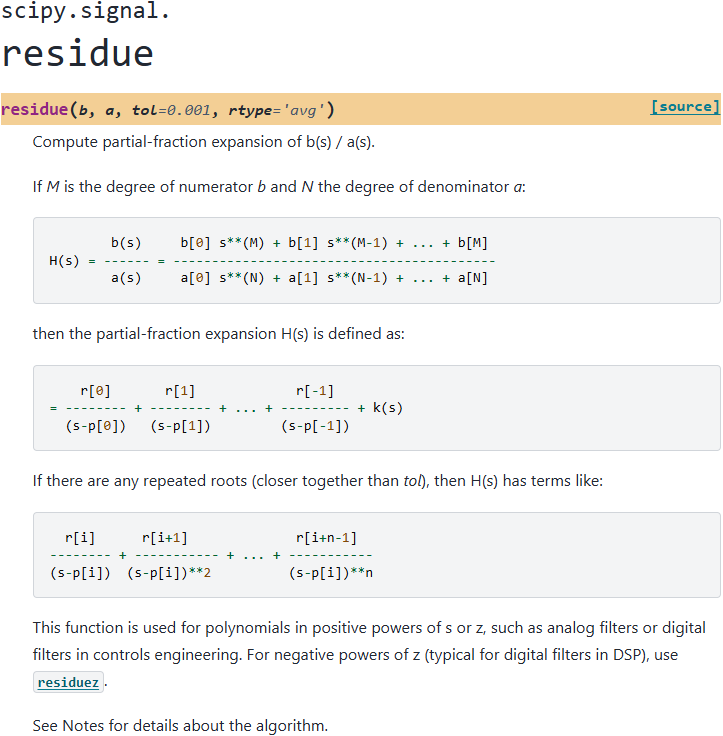
\includegraphics[width=10cm]{7.2.6-1-1.png}
\end{figure}
\begin{figure}[ht]
\centering
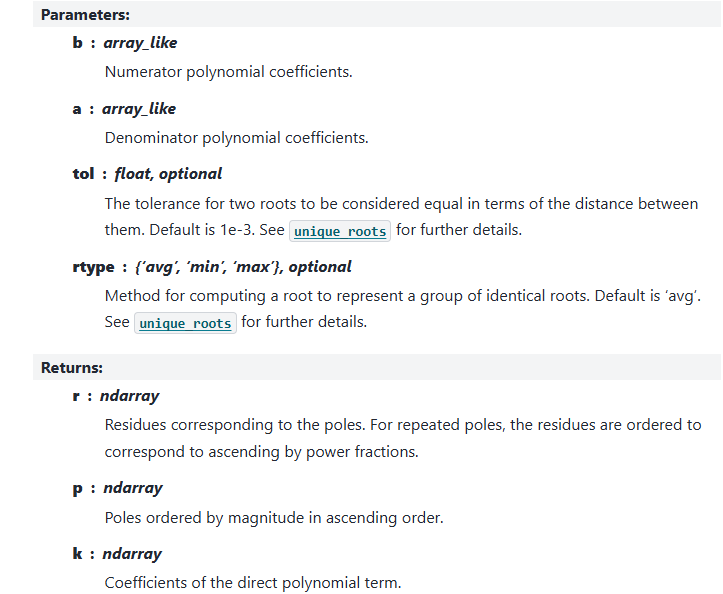
\includegraphics[width=10cm]{7.2.6-1-2.png}
\end{figure}

~

~

~

~

\begin{example}
如信号$x\left( t \right) $的拉普拉斯变换$X\left( s \right) =\frac{s+2}{s^3+4s^2+3s}$,求$x\left( t \right) $。
\end{example}

\begin{python}
import numpy as np
from scipy import signal

import fractions
np.set_printoptions(formatter={'all':lambda x: str(fractions.Fraction(x).limit_denominator())})

b = [1,2]
a = [1,4,3,0]
r,p,k = signal.residue(b, a)

=====output=====
b = [2/3 -1/2 -1/6]
p = [0 -1 -3]
k = []
\end{python}

注意,我们导入fractions模块,并设置np的值都以分数形式打印。
得到信号:
\[
x\left( t \right) =\frac{2}{3}+\left( -\frac{1}{2} \right) e^{-t}+\left( -\frac{1}{6} \right) e^{-3t} \qquad t\geqslant 0
\]
由于极点都是实数解,且都小于0,所以$x\left( t \right) $最终是指数衰减。

~

\begin{example}
如信号$x\left( t \right) $的拉普拉斯变换$X\left( s \right) =\frac{s^2-2s+1}{s^3+3s^2+4s+2}$,求$x\left( t \right) $。
\end{example}

\begin{python}
import numpy as np
from scipy import signal

b = [1,-2,1]
a = [1,3,4,2]
r,p,k = signal.residue(b, a)

=====output=====
r = [ 4. +0.j -1.5+2.j -1.5-2.j]
p = [-1.+0.j -1.+1.j -1.-1.j]
k = []
\end{python}

得到一个实数极点和一对共轭对极点:
\[
\begin{cases}
	p_1=-1\\
	c_1=4\\
\end{cases} \qquad \begin{cases}
	p_2,\bar{p}_2=1\pm i\\
	c_2,\bar{c}_2=-\frac{2}{3}\pm 2i\\
\end{cases}
\]
最终得到信号:
\begin{align*}
x\left( t \right) &=4e^{-t}+c_2e^{p_2t}+\bar{c}_2e^{\bar{p}_2t}=4e^{-t}+2\left| c_2 \right|e^t\cos \left( t+\angle c_2 \right) \\
&=4e^{-t}+5e^{-t}\cos \left( t+126.87^{\circ} \right)
\end{align*}




